\documentclass[xcolor=dvipsnames]{beamer}
%\documentclass[aspectratio=169,xcolor=dvipsnames]{beamer}

%=================================================================================
% Document information
\def\firstname{Marc}
\def\familyname{Henry de Frahan}
\def\FileAuthor{\firstname~\familyname}
\def\FileTitle{ParCFD 2017}
\def\FileSubject{ParCFD 2017}
\def\FileKeyWords{\firstname~\familyname, \FileSubject, \FileTitle}

%=================================================================================
% Preamble
%=================================================================================
% PACKAGES
\usepackage{amsmath}
\usepackage{amssymb}
\usepackage{amsfonts}
\usepackage{wasysym} % for circles
\usepackage{graphicx}
\usepackage[utf8]{inputenc}
%\usepackage[usenames,dvipsnames]{color}
\usepackage{textcomp}
\usepackage{alltt}
%\usepackage{subfigure}
\usepackage{latexsym}
\usepackage{eurosym}
\usepackage{verbatim}
\usepackage{epstopdf}         % if you want to use .eps and .jpeg in the same document (compile with pdflatex directly)
\usepackage{array}            % permet d'utiliser m{width} dans l'env tabular
\usepackage[english]{babel}
\usepackage{multirow}
\usepackage{algorithmic}
\usepackage{units}
\usepackage{nicefrac}
\usepackage{natbib} 
\usepackage{appendix}
%\usepackage{chapterbib}
\usepackage{booktabs}
\usepackage{pdfpages}        % to include pdf pages into the doc \includepdf[pages={1}]{myfile.pdf}
\usepackage{layout}          % then \layout in the document to get the layout numbers
\usepackage{hyperref}        % Hyper references for the document
\usepackage{subcaption}
\hypersetup{
  colorlinks=true,       % false: boxed links; true: colored links
  breaklinks=true,    % permet le retour à la ligne dans les liens trop longs
  linkcolor=black,       % color of internal links (red)
  citecolor=black,       % color of links to bibliography (green)
  filecolor=black,       % color of file links (magenta)
  urlcolor=black,        % color of external links (cyan)
  pdftitle={\FileTitle},
  pdfauthor={\FileAuthor},
  pdfsubject={\FileSubject},
  pdfkeywords={\FileKeyWords}}

% BEAMER specific
\mode<article>{\usepackage{fullpage}}
\mode<presentation>
{
  \usetheme{default}
  \usecolortheme{default} % beetle, lily, beaver
}
\usepackage{tikz}
\usepackage{mdwlist}
\usepackage{moreverb}
\usepackage{etex}   % this is a dodgy fix for using lpic: http://www.tex.ac.uk/cgi-bin/texfaq2html?label=noroom
\usepackage{lpic}
\usepackage[absolute,overlay]{textpos} % for absolute positioning on page
\setbeamertemplate{navigation symbols}{}
\setbeamertemplate{footline}{\leavevmode% 
  \hfill\hbox{% 
    \begin{beamercolorbox}[wd=1.0\paperwidth,ht=2.25ex,dp=1ex,left]{date in head/foot}% 
      \scriptsize \hspace*{1ex} \insertframenumber{} %
    \end{beamercolorbox}}% 
  \vskip0pt%
}
\beamertemplatetransparentcovereddynamic
\beamertemplateballitem
\beamertemplatesolidbuttons
\usefonttheme[onlymath]{serif}
\setbeamercovered{invisible} % http://tex.stackexchange.com/questions/53860/can-i-tell-beamer-that-uncover-should-be-invisible-not-merely-grayed-out


%=================================================================================
% Useful commands
\newcommand{\minimum}[1]{\mathop{\textrm{min}}_{#1}\,}
\newcommand{\maximum}[1]{\mathop{\textrm{max}}_{#1}\,}
\newcommand{\argmin}[1]{\mathop{\textrm{arg min}}_{#1}\,}
\newcommand{\dg}{\textsc{dg}}
\newcommand{\bs}{\boldsymbol}
\newcommand{\mbf}[1]{\mathbf{#1}}
\newcommand{\com}[1]{\textcolor{red}{#1}\marginpar{\textcolor{red}{\Large $/!\backslash$}}}
\newcommand{\pfrac}[2]{\frac{\partial#1}{\partial#2}}
\newcommand{\dpfrac}[2]{\dfrac{\partial#1}{\partial#2}}
\newcommand{\ufrac}[2]{\frac{\ud{}#1}{\ud{}#2}}
\newcommand{\dufrac}[2]{\dfrac{\ud{}#1}{\ud{}#2}}
\newcommand{\wt}[1]{\widetilde{#1}}
\newcommand{\ol}[1]{\overline{#1}}
\newcommand{\avg}[1]{\left\{\!\!\left\{#1\right\}\!\!\right\}}
\newcommand{\jmp}[1]{\left[\!\left[#1\right]\!\right]}
\newcommand{\hr}{\textsc{hr}}
\newcommand{\xjl}{x_{j-\nicefrac{1}{2}}}
\newcommand{\xjr}{x_{j+\nicefrac{1}{2}}}
\newcommand{\xRl}{x_{I-\nicefrac{1}{2}}}
\newcommand{\xRr}{x_{I+\nicefrac{1}{2}}}
\newcommand{\xLl}{x_{(I-1)-\nicefrac{1}{2}}}
\newcommand{\xLr}{x_{(I-1)+\nicefrac{1}{2}}}
\newcommand{\ud}{\,\mathrm{d}}
\newcommand{\dgm}{\textsc{dgm}}
\newcommand{\fem}{\textsc{fem}}
\newcommand{\fvm}{\textsc{fvm}}
\newcommand{\cpu}{\textsc{cpu}}
\newcommand{\gpu}{\textsc{gpu}}
\newcommand{\gpub}{\textsc{gpublas}}
\newcommand{\blas}{\textsc{blas}}
\newcommand{\cublas}{\textsc{cublas}}
\newcommand{\cuda}{\textsc{cuda}}
\newcommand{\pcpu}{$P_{\cpu{}}$}
\newcommand{\pgpu}{$P_{\gpu{}}$}
\newcommand{\pgpub}{$P_{\gpub{}}$}
\newcommand{\pcpuc}{\textcolor{red}{$P_{\cpu{}}$}}
\newcommand{\pgpuc}{\textcolor{olivegreen}{$P_{\gpu{}}$}}
\newcommand{\pgpubc}{\textcolor{blue}{$P_{\gpub{}}$}}
\newcommand{\bth}{$B_{\text{theo}}$}
\newcommand{\bpr}{$B_{\text{pract}}$}
\newcommand{\bcpu}{$B_{\text{\cpu{}}}$}
\newcommand{\bgpu}{$B_{\text{\gpu{}}}$}
\newcommand{\bgpub}{$B_{\text{\gpub{}}}$}
\newcommand{\e}[1]{\ensuremath{\times 10^{#1}}}
\newcommand{\tabcn}[1]{\multicolumn{1}{c}{\makebox[0.65cm]{\tiny #1}}} % for a tabular workaround
\renewcommand*{\thesubfigure}{}  % Gets rid of the subfigure counter!!
\newcommand{\alf}{Alfvén}
\newcommand{\els}{Elsässer}
% Needed for the title page:
\newcommand{\HRule}{\rule{\linewidth}{0.5mm}}
\renewcommand{\topfraction}{0.85}
\renewcommand{\textfraction}{0.1}
\renewcommand{\floatpagefraction}{0.75}
% Needed for the natbib bibliography style
%\newcommand*{\newblock}{}
%% \bibpunct[<optional>]{}{}{;}{}{}{} 
% To put a box around a figure
\setlength\fboxsep{0pt}
\setlength\fboxrule{0.5pt}
\def\CC{{C\nolinebreak[4]\hspace{-.05em}\raisebox{.4ex}{\tiny\bf ++}}}

% increase space in underbrace env (http://tex.stackexchange.com/questions/13843/vertical-spacing-with-underbrace-command)
\newcommand*\mystrut[1]{\vrule width0pt height0pt depth#1\relax}

% https://tex.stackexchange.com/questions/33401/a-version-of-colorbox-that-works-inside-math-environments
\newcommand{\highlight}[2][yellow]{\mathchoice%
  {\colorbox{#1}{$\displaystyle#2$}}%
  {\colorbox{#1}{$\textstyle#2$}}%
  {\colorbox{#1}{$\scriptstyle#2$}}%
  {\colorbox{#1}{$\scriptscriptstyle#2$}}}%

%=================================================================================
% Define some colors
\definecolor{violetred}{rgb}{0.78,0.08,0.52}
\definecolor{olivegreen}{rgb}{0.2,0.6,0.0}
\definecolor{darkgray}{rgb}{0.95,0.95,0.95}
\definecolor{mypurple}{rgb}{0.76,0.06,0.76}
\definecolor{greenyellow}{rgb}{0.76,0.76,0.06}
\definecolor{gold}{HTML}{FFD700} 
\definecolor{IMnumber}{HTML}{AFB9DB}

% From http://www.google.com/url?sa=t&rct=j&q=&esrc=s&source=web&cd=1&ved=0CFcQFjAA&url=http%3A%2F%2Fwww.perceptualedge.com%2Farticles%2Fvisual_business_intelligence%2Frules_for_using_color.pdf&ei=TioYUPL8GMPl0QHhqICQAQ&usg=AFQjCNGA9t1pGae49wQ0DVhaSNcAk6oLyA&sig2=QuA9D9nierTbqn3djCyyPQ
\definecolor{c1med}{HTML}{F15A60} % red
\definecolor{c2med}{HTML}{7AC36A} % green
\definecolor{c3med}{HTML}{5A9BD4} % blue
\definecolor{c4med}{HTML}{FAA75B} % orange
\definecolor{c5med}{HTML}{9E67AB} % purple
\definecolor{c6med}{HTML}{CE7058} % burgundy
\definecolor{c7med}{HTML}{D77FB4} % magenta
\definecolor{c8med}{HTML}{737373} % grey

\definecolor{c1brt}{HTML}{EE2E2F} % red     
\definecolor{c2brt}{HTML}{008C48} % green   
\definecolor{c3brt}{HTML}{185AA9} % blue    
\definecolor{c4brt}{HTML}{F47D23} % orange  
\definecolor{c5brt}{HTML}{662C91} % purple  
\definecolor{c6brt}{HTML}{A21D21} % burgundy
\definecolor{c7brt}{HTML}{B43894} % magenta 
\definecolor{c8brt}{HTML}{010202} % black

\newcommand{\tcb}[2]{\textcolor{c#1brt}{#2}}
\newcommand{\tcm}[2]{\textcolor{c#1med}{#2}}

%=================================================================================
% Tikz special stuff (do after color definitions)
\usetikzlibrary{decorations.pathreplacing}
\usetikzlibrary{calc}
\usetikzlibrary{decorations.shapes}
\usetikzlibrary{decorations.pathmorphing}
\tikzset{paint/.style={fill=red}, decorate with/.style={decorate,decoration={shape backgrounds,shape=#1,shape size=3pt}}}
\tikzset{dotr/.style={fill=c1brt,circle,minimum size=3pt}}
\tikzset{dotb/.style={fill=c3brt,circle,minimum size=3pt}}
\tikzset{dotrr/.style={fill=c1brt,circle,minimum size=0.2cm,inner sep=0}}
\usetikzlibrary{positioning}
\usetikzlibrary{shapes}
\usetikzlibrary{snakes}
%fill=red,circle,minimum size=3pt
\usepackage{pgfkeys}
\usepackage{pgf,pgfarrows,pgfnodes,pgfautomata,pgfheaps,pgfshade}

%=================================================================================
% Environments 
% Theorem environments (from http://www.math.uiuc.edu/~hildebr/tex/theorems.html)
\newtheorem{thm}{Théorème}[section]
\newtheorem{cor}[thm]{Corollary}
\newtheorem{lem}[thm]{Lemma}
%\theoremstyle{remark}
\newtheorem{rem}[thm]{Remark}
%\theoremstyle{definition}
%\newtheorem{def}[thm]{Definition}

% Tight lists
\newenvironment{tight-itemize}
{\begin{itemize}
  \setlength{\itemsep}{1pt}
  \setlength{\parskip}{0pt}
  \setlength{\parsep}{0pt}}
{\end{itemize}}
\newenvironment{tight-enumerate}
{\begin{enumerate}
  \setlength{\itemsep}{1pt}
  \setlength{\parskip}{0pt}
  \setlength{\parsep}{0pt}}
{\end{enumerate}}
\newenvironment{tight-description}
{\begin{description}
  \setlength{\itemsep}{1pt}
  \setlength{\parskip}{0pt}
  \setlength{\parsep}{0pt}}
{\end{description}}

%=================================================================================
% For code inclusion
\usepackage{listings}
\lstset{
language=c,                        % choose the language of the code
basicstyle=\tiny,                  % the size of the fonts that are used for the code
backgroundcolor=\color{white}, %\color{darkgray},  % choose the background color. You must add \usepackage{color}
showspaces=false,               % show spaces adding particular underscores
showstringspaces=false,         % underline spaces within strings
showtabs=false,                 % show tabs within strings adding particular underscores
frame=none,                     % adds a frame around the code
tabsize=1,                      % sets default tabsize to 4 spaces
captionpos=t,                   % sets the caption-position to bottom
breaklines=true,                % sets automatic line breaking
numbers=none,                   % where to put the line-numbers
numberstyle=\tiny,              % the size of the fonts that are used for the line-numbers
stepnumber=1,                   % the step between two line-numbers. If it's 1 each line will be numbered
numbersep=5pt,                  % how far the line-numbers are from the code
keywordstyle=\color[rgb]{0,0,1},
commentstyle=\color[rgb]{0.133,0.545,0.133},
stringstyle=\color[rgb]{0.627,0.126,0.941},
morekeywords={scalar,dim3, end}      % if you want to add more keywords to the set
}

%=================================================================================
% For media inclusion
%\usepackage{movie15}
%\usepackage{media9}
\usepackage{multimedia}


\title[]{}
\author[Marc T. Henry de Frahan]{Marc T. Henry de Frahan}
\date{\today}

\begin{document}
\presentation

%=================================================================================
% Title page
\bgroup
\setbeamertemplate{background}{\begin{tikzpicture}\node at (0,0){};\node[inner sep=0,opacity=1]{
\includegraphics[width=1\paperwidth,height=1\paperheight]{./figs/ecp_title_4x3.jpg}};\end{tikzpicture}}
\frame[plain]{
  \hspace*{0.cm}\begin{minipage}{1\textwidth}
    \vspace*{-0.7cm}                                      
    \textbf{\textcolor{black}{\LARGE A-priori analysis of joint PDF of mixture fraction and progress variable trained using machine learning techniques}}\par
    \vspace*{2.cm}
    \textbf{\textcolor{black}{\large \mbox{M. T. Henry de Frahan$^\text{a}$}, S. Yellapantula$^\text{a}$,}}\\[0.1cm]
    \textbf{\textcolor{black}{\large R. King$^\text{b}$, M. Day$^\text{c}$, R. Grout$^\text{a}$}}\\[0.1cm]
    \textbf{\textcolor{black}{\footnotesize November 20, 2018}}\\
    \textit{\scriptsize\textcolor{black}{$^\text{a}$High Performance Algorithms and Complex Fluids, NREL}}\\[-0.1cm]
    \textit{\scriptsize\textcolor{black}{$^\text{b}$Complex Systems Simulation and Optimization Group, NREL}}\\[-0.1cm]
    \textit{\scriptsize\textcolor{black}{$^\text{c}$Center for Computational Sciences and Engineering, LBNL}}\\[0.2cm]
  \end{minipage}
  % \begin{textblock*}{\paperwidth}[0,0](0.\paperwidth,0.25\paperheight)
  %   \includegraphics[width=\paperwidth]{./figs/wallhump_white.png}
  % \end{textblock*}
  \setcounter{framenumber}{0}
  \begin{textblock*}{4.cm}[1,1](0.39\paperwidth,.91\paperheight)
    
\includegraphics[width=1\textwidth]{./figs/logos/nrel.jpg}
  \end{textblock*}
  \begin{textblock*}{2.3cm}[1,1](0.67\paperwidth,.9\paperheight)
    
\includegraphics[width=1\textwidth]{./figs/logos/lbl.png}
  \end{textblock*}
  }
\egroup

% Everyone has the same background
\bgroup
\setbeamertemplate{background}{\begin{tikzpicture}\node at (0,0){};\node[inner sep=0,opacity=1]{
\includegraphics[width=1\paperwidth,height=1\paperheight]{./figs/ecp_main_4x3.jpg}};\end{tikzpicture}}

% ================================================================================
% Motivation/objective
\frame{
  \frametitle{Presumed PDF modeling for large eddy simulations of combustion processes.}
  \setlength{\fboxsep}{4pt}
  \begin{align*}
    \highlight[c1med!70]{\wt{\dot{\omega}}} = \int \highlight[c2med!70]{\langle \dot{\omega} | Z, c \rangle \strut} \quad \highlight[c3med!70]{\strut P(Z,c | \wt{Z}, \wt{Z''}, \wt{c}, \wt{c''})} \ud Z \ud c
  \end{align*}
  $\highlight[c1med!70]{\wt{\dot{\omega}}}$ is the Favre filtered progress variable source term\\[0.2cm]
  $\highlight[c2med!70]{\langle \dot{\omega} | Z, c \rangle \strut}$ is the conditional means of $\dot{\omega}$\\[-0.1cm]
  \mbox{\hphantom{$\highlight[c2med!70]{\langle \dot{\omega} | Z, c \rangle \strut}$} often modeled based on physical theories}\\
  \mbox{\hphantom{$\highlight[c2med!70]{\langle \dot{\omega} | Z, c \rangle \strut}$} computed from the data in this work}\\[0.2cm]
  $\highlight[c3med!70]{\strut P(Z,c | \wt{Z}, \wt{Z''}, \wt{c}, \wt{c''})}$ is the density weighted PDF\\[-0.1cm]
  \mbox{\hphantom{$\highlight[c3med!70]{\strut P(Z,c | \wt{Z}, \wt{Z''}, \wt{c}, \wt{c''})}$}} most models use $P(Z,c) = \beta-\beta/\beta-\delta$\\[0.5cm]
  \mbox{\textbf{Can we provide accurate PDF models using machine learning?}}
}

% ================================================================================
% DNS
\frame{
  \frametitle{A data snapshot at $t=0.0626\unit{s}$ of the Low Swirl Burner DNS was used for ML training.}
  \vspace*{0.2cm}
  \structure{Reacting flow DNS details}\\
  \hspace*{0.5cm}LMC code with adaptive mesh refinement (LBNL)\\
  \hspace*{0.5cm}3 levels of refinement (finest $\Delta x \approx 0.1\unit{mm}$)\\
  \hspace*{0.5cm}DRM 19 chemical mechanism for finite rate kinetics\\[0.1cm]
  \hspace{0.5cm}\begin{minipage}[c]{0.3\textwidth}%
    \begin{center}%
      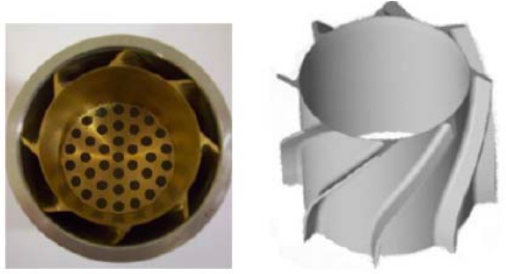
\includegraphics[width=\textwidth]{./figs/lsb_nozzle.png}\\%
      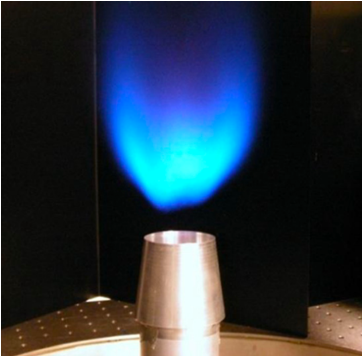
\includegraphics[width=\textwidth]{./figs/lsb_exp.png}
    \end{center}%
  \end{minipage}\hspace*{1.4cm}%
  \begin{minipage}[c]{0.4\textwidth}%
    \begin{center}%
      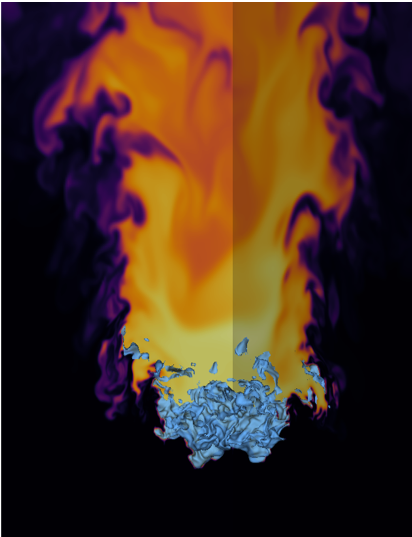
\includegraphics[width=\textwidth]{./figs/lsb_dns.png}
    \end{center}%
  \end{minipage}%
  \begin{textblock*}{100mm}(0.83\paperwidth,.5\paperheight)%
    {\scriptsize $p=1\unit{atm}$\\%
      Burner: CH4/air\\
      Co-flow: air\\
      $\Phi = 0.7$\par}
  \end{textblock*}
  \begin{textblock*}{100mm}(0.49\paperwidth,.92\paperheight)%
    {\tiny \color{white} Contours of $T~[\unit{K}]$\\%
      iso-surface of $\dot{\omega}$ (blue)\par}
  \end{textblock*}
  \begin{textblock*}{100mm}(0.6cm,.945\paperheight)%
    {\tiny M. Day et. al, Combust. Flame 159 (1) (2012) 275–290\\%
      Cheng, R. K., P. Combust. Inst. 28.1 (2000): 1305-1313\par}
  \end{textblock*}
}

\frame{
  \frametitle{The data for ML training is extracted from the LSB DNS.}
  \vspace*{0.4cm}
  Sub-volumes equi-spaced in DNS ($1146 \times 1146 \times 51$ cells)\\
  Box filter with $\ol{\Delta} = 32 \Delta x$, spaced at $8\Delta x$ in each sub-volume\\[0.2cm]
  \begin{center}
    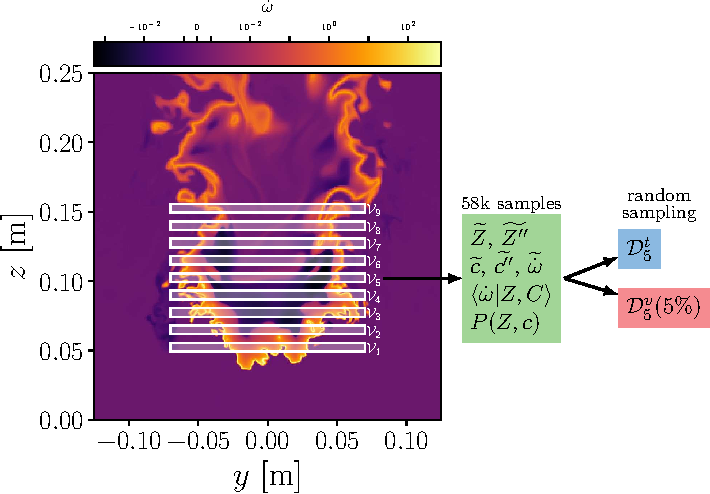
\includegraphics[width=0.9\textwidth]{./figs/gen_data.pdf}  
  \end{center}

}

\frame{
  \frametitle{Distribution of sample moments (ML inputs) illustrate the two different burning regimes ($\mathcal{V}_3$, $z_3=0.0775\unit{m}$).}
  \vspace*{0.5cm}
  Premixed burning of the fuel-air from the nozzle $\wt{Z}=1$ and $\wt{c} = 0.2$\\
  Non-premixed burning of the products (intermediate $\wt{Z}$ and $\wt{c}$)
  \begin{figure}%
    \centering%
    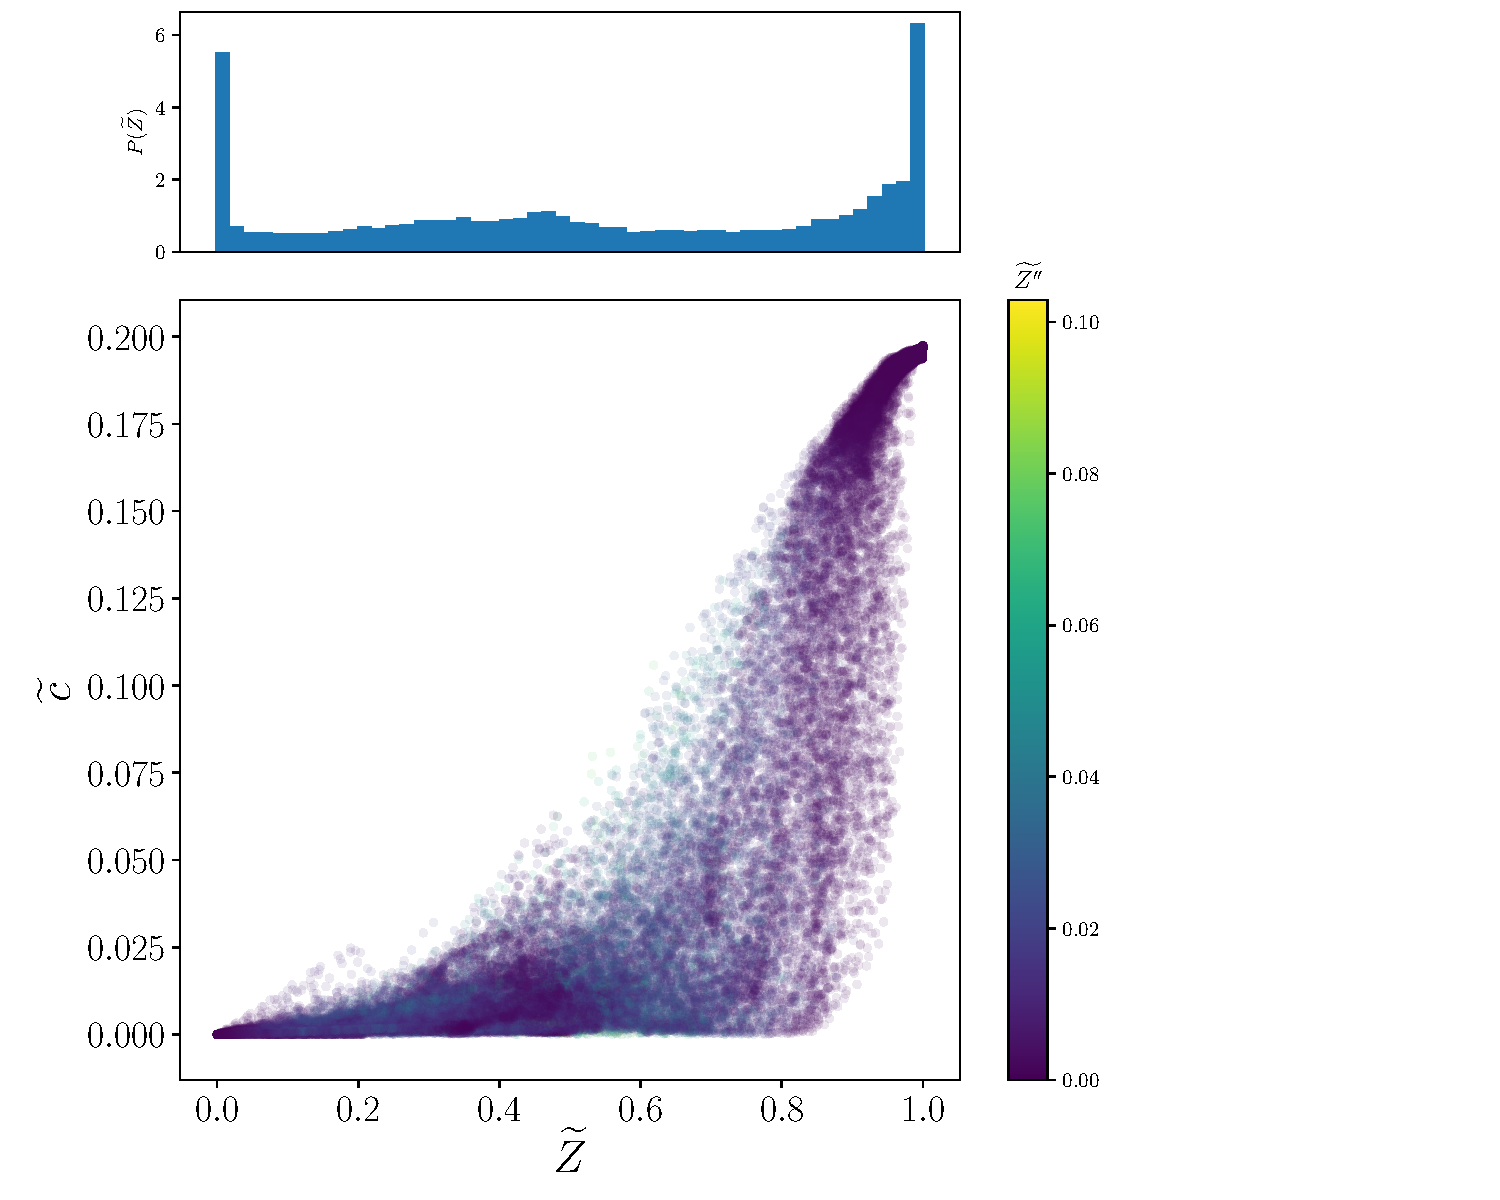
\includegraphics[page=1, height=0.5\textwidth, trim=0.0cm 0cm 6.4cm 0cm, clip]{./figs/inputs_dice_0004.pdf}%
    \includegraphics[page=2, height=0.5\textwidth, trim=1.0cm 0cm 2.4cm 0cm, clip]{./figs/inputs_dice_0004.pdf}
  \end{figure}%
}

\frame{
  \frametitle{Examples of $P(Z,c)$ and $\langle \dot{\omega} | Z, c \rangle$ for increasing $\wt{\dot{\omega}}$ illustrate the wide range of observed shapes.}
  \begin{figure}[!tbp]%
    \centering%
    \begin{subfigure}[t]{0.48\textwidth}%
      \includegraphics[page=9,width=\textwidth]{./figs/pdfs_dice_0004.pdf}%
      %\caption{Marginal $P(Z,c)$ as a function of $Z$.}%
    \end{subfigure}\hfill%
    \begin{subfigure}[t]{0.48\textwidth}%
      \includegraphics[page=10,width=\textwidth]{./figs/pdfs_dice_0004.pdf}%
      %\caption{Marginal $P(Z,c)$ as a function of $c$.}%
    \end{subfigure}\\%
    \begin{subfigure}[t]{0.48\textwidth}%
      \includegraphics[page=11,width=\textwidth]{./figs/pdfs_dice_0004.pdf}%
      %\caption{Marginal conditional means of $\dot{\omega}$ as a function of $Z$.}%
    \end{subfigure}\hfill%
    \begin{subfigure}[t]{0.48\textwidth}%
      \includegraphics[page=12,width=\textwidth]{./figs/pdfs_dice_0004.pdf}%
      % \caption{Marginal conditional means of $\dot{\omega}$ as a function of $c$.}%
    \end{subfigure}%
    \caption{Examples of $P(Z,c)$ and $\langle \dot{\omega} | Z, c \rangle$ for increasing $\wt{\dot{\omega}}$. Red solid: $\wt{\dot{\omega}} = 0$ ($\wt{Z} = 0$, $\wt{Z''} = 0$, $\wt{c} = 0$, $\wt{c''} = 0$); green dashed: $\wt{\dot{\omega}} = 0.03$ ($\wt{Z}  =0.4$, $\wt{Z''}=0.006$, $\wt{c}  =0.03$, $\wt{c''}=0.0006$); blue dash-dotted: $\wt{\dot{\omega}} = 7.4$ ($\wt{Z}  =0.7$, $\wt{Z''}=0.01$, $\wt{c}  =0.08$, $\wt{c''}=0.003$); orange short dashed: $\wt{\dot{\omega}} = 42.2$ ($\wt{Z}  =0.9$, $\wt{Z''}=0.003$, $\wt{c}  =0.12$, $\wt{c''}=0.005$).}\label{fig:pdfs}%
\end{figure}%
}

% ================================================================================
% ML methods
\frame{
  \frametitle{We evaluate different machine learning algorithms.}
  \begin{minipage}[t]{0.32\textwidth}%
    \begin{center}%
      {\footnotesize \structure{Traditional ML}}\\%
      \begin{figure}%
        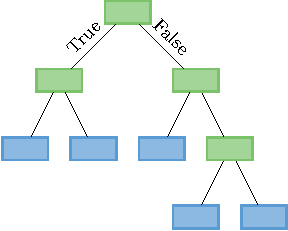
\includegraphics[height=0.6\textwidth]{./figs/rf.pdf}%
      \end{figure}\vspace{-0.5cm}%
      {\flushleft\footnotesize Random forests:\\%
        \scriptsize\hspace*{0.2cm}estimators = 100\\%
        \hspace*{0.2cm}depth = 30\par}%
    \end{center}%
  \end{minipage}\hfill\vrule width 0.2pt \hfill%
  \begin{minipage}[t]{0.32\textwidth}%
    \begin{center}%
      {\footnotesize \structure{Deep learning}}\\%
      \begin{figure}%
        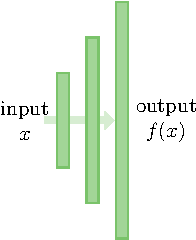
\includegraphics[height=0.6\textwidth]{./figs/dnn.pdf}%
      \end{figure}\vspace{-0.5cm}%
      {\flushleft\footnotesize Deep neural network:\\%
        \scriptsize\hspace*{0.2cm}3 layers: $[ 256, 512, 2048]$\\%
        \hspace*{0.2cm}Leaky ReLU activations\\%
        \hspace*{0.2cm}Softmax output\\%
        \hspace*{0.2cm}Binary cross-entropy loss\\%
        \hspace*{0.2cm}500 epochs\\
        \hspace*{0.2cm}ADAM optimizer\par%
      }%
    \end{center}%
  \end{minipage}\hfill\vrule width 0.2pt \hfill%
  \begin{minipage}[t]{0.32\textwidth}%
    \begin{center}%
      {\footnotesize \structure{Unsupervised, generative}}\\%      
      \begin{figure}%
        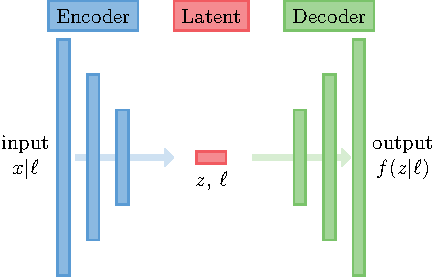
\includegraphics[height=0.6\textwidth]{./figs/cvae.pdf}%
      \end{figure}\vspace{-0.5cm}%
      {\flushleft \footnotesize Variational autoencoder:\\%
        \scriptsize \hspace*{0.2cm}encoder: $[ 2048, 512, 256]$\\%
        \hspace*{0.2cm}decoder: $[ 256, 512, 2048]$\\%
        \hspace*{0.2cm}latent dimension: 10\\%
        \hspace*{0.2cm}leaky ReLU activations\\%
        \hspace*{0.2cm}softmax output\\%
        \hspace*{0.2cm}BCE and KL div. loss\\%
        \hspace*{0.2cm}500 epochs\\
        \hspace*{0.2cm}ADAM optimizer\par%
      }%
    \end{center}%
  \end{minipage}\\[0.5cm]%
}


% ================================================================================
% Results
\frame{
  \frametitle{We evaluate different model development strategies using the following tests and metrics.}
  \vspace*{0.3cm}
  \structure{Model tests}\\
  \hspace*{1cm}1. Trained and evaluated at $z=0.0775\unit{m}$\\
  \hspace*{1cm}\mbox{2. Trained on every other volume, evaluated on other regions}\\[0.5cm]
  \structure{Metric for $P(Z,c)$ (Jensen-Shannon divergence)}
  \begin{align*}
    &J(Q||R)= \frac{1}{2} \left( D(Q || M) + D(R || M)\right)\\
    &\text{where }M = \nicefrac{1}{2}(Q+R) \quad\text{and } D(Q||R) = \sum_{i=1}^n R(i) \ln{\left( \nicefrac{R(i)}{Q(i)} \right)}
  \end{align*}
  \structure{Metric for $\wt{\dot{\omega}}$ (normalized RMSE)}
  \begin{align*}
    \text{RMSE}(\wt{\dot{\omega}}) = \frac{1}{\wt{\dot{\Omega}}}\sqrt{ \frac{1}{|\mathcal{D}|}\sum_{i=1}^{|\mathcal{D}|}\left( \epsilon(\wt{\dot{\omega}}_i) \right)^2}
  \end{align*}
  Metrics are evaluated on a validation set (not used for training).
}

\frame{
  \frametitle{Machine learning models accurately capture the complexity in the PDFs.}
  \begin{align*}
    \setlength{\fboxsep}{4pt}
    \wt{\dot{\omega}} = \int \langle \dot{\omega} | Z, c \rangle \ \highlight[c3med!70]{\strut P(Z,c | \wt{Z}, \wt{Z''}, \wt{c}, \wt{c''})} \ud Z \ud c
  \end{align*}
  \begin{figure}%
  \centering%
  \begin{subfigure}[t]{0.48\textwidth}%
    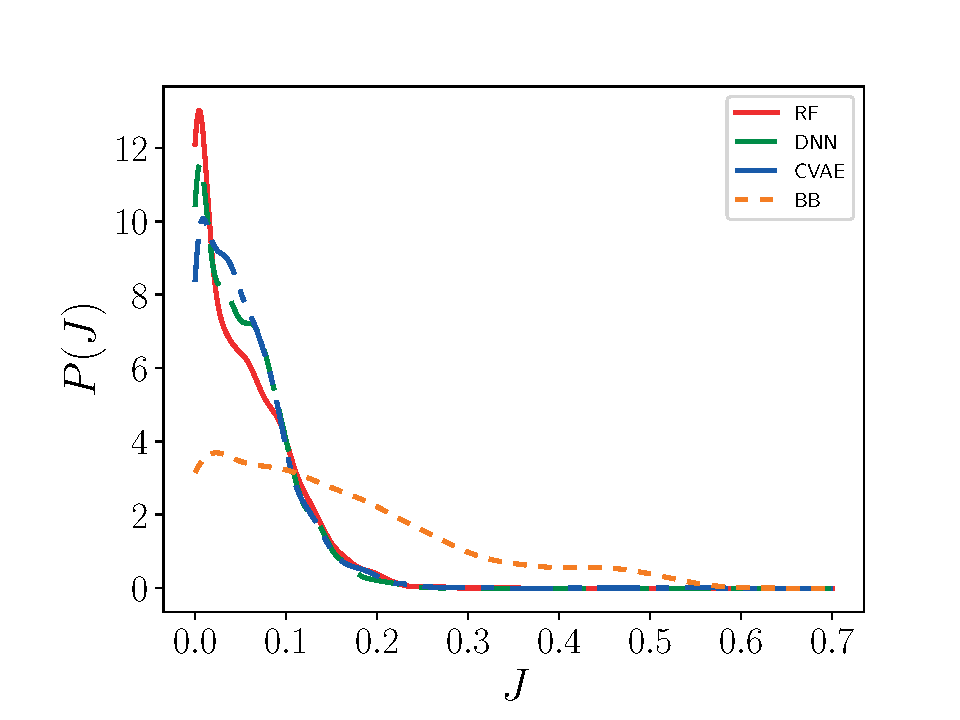
\includegraphics[page=1,width=\textwidth, trim=0.5cm 0cm 1.5cm 1.3cm, clip=true]{./figs/jsd_dice_0004.pdf}%
    %\caption*{Probability density function of $J$.}\label{fig:jsd_pdf}%
  \end{subfigure}\hfill%
  \begin{subfigure}[t]{0.48\textwidth}%
    \includegraphics[page=2,width=\textwidth, trim=0.5cm 0cm 1.5cm 1.3cm, clip=true]{./figs/jsd_dice_0004.pdf}%
    %\caption*{Cumulative density function of $J$.}\label{fig:jsd_cdf}%
  \end{subfigure}%
  %\caption*{Red solid: RF; green dashed: DNN; blue dash-dotted: CVAE; orange short dashed: $\beta-\beta$ model.}\label{fig:jsd}%
\end{figure}%
}

\frame{
  \frametitle{Leading to accurate predictions of the filtered reaction rates using ML models.}
  \begin{align*}
    \setlength{\fboxsep}{4pt}
    \highlight[c1med!70]{\wt{\dot{\omega}}} = \int \langle \dot{\omega} | Z, c \rangle P(Z,c | \wt{Z}, \wt{Z''}, \wt{c}, \wt{c''}) \ud Z \ud c
  \end{align*}
  \begin{figure}[!tbp]%
  \centering%
  \begin{subfigure}[t]{0.48\textwidth}%
    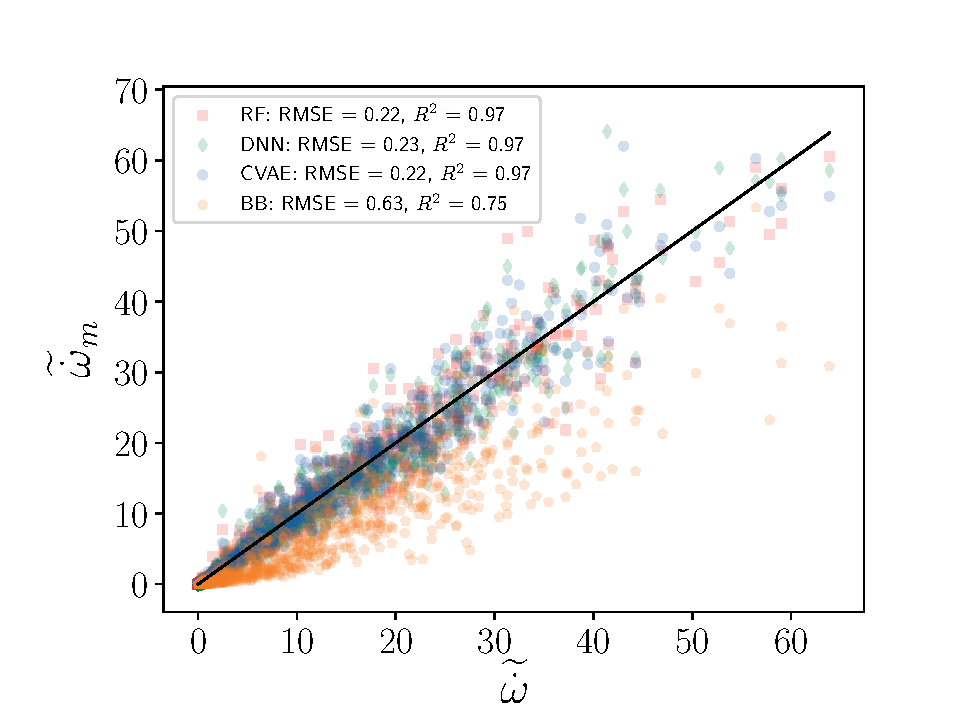
\includegraphics[page=1,width=\textwidth, trim=0.5cm 0cm 1.5cm 1.3cm, clip=true]{./figs/convolution_dice_0004.pdf}%
    %\caption*{$\wt{\dot{\omega}}$ predictions.}\label{fig:convolution_scatter}%
  \end{subfigure}\hfill%
  \begin{subfigure}[t]{0.48\textwidth}%
    \includegraphics[page=2,width=\textwidth, trim=0.5cm 0cm 1.5cm 1.3cm, clip=true]{./figs/convolution_dice_0004.pdf}%
    %\caption*{PDF of $\epsilon(\wt{\dot{\omega}})$.}\label{fig:convolution_pdf}%
  \end{subfigure}%
  %\caption*{Red squares and solid: RF; green diamonds and dashed: DNN; blue circles and dash-dotted: CVAE; orange pentagons and short dashed: $\beta-\beta$ model.}\label{fig:convolution}%
\end{figure}%
}

\frame{
  \frametitle{ML models achieve similar performance but the RF model is large and exhibits high evaluation times.}
  \begin{center}
    \begin{tabular}{lccccc}
      \toprule
      model & $J_{90}$ & $t_m~[\unit{ms}]$ & RMSE$(\wt{\dot{\omega}})$& $R^2(\wt{\dot{\omega}})$ & Size (MB)\\
      \midrule
      RF            & 0.12 & 0.932 & 0.22 & 0.97 & 82107 \\
      DNN           & 0.11 & 0.036 & 0.23 & 0.97 & 27    \\
      CVAE          & 0.12 & 0.038 & 0.22 & 0.97 & 36    \\
      $\beta-\beta$ & 0.35 & 1.178 & 0.63 & 0.75 & {--}  \\
      \bottomrule
    \end{tabular}
  \end{center}
  \vspace*{0.5cm}
  {\footnotesize $J_{90}$ is the $90^\text{th}$ percentile of $J(P||P_m)$\\
  $t_m = \frac{1}{n_t |\mathcal{D}_3^v|} \sum_{i=1}^{n_t} \text{time to evaluate } m(\mathcal{D}_3^v)$\\
  \mbox{$\beta-\beta$ model evaluated using SciPy, RF with scikit-learn, DNN/CVAE with PyTorch}}\par
}

\frame{
  \frametitle{ML models are able to interpolate to other regions of the domain (trained on every other region).}
  Training data: $\mathcal{D}^t = \bigcup\limits_{i=1, 3, 5, 7, 9} \mathcal{D}_i^t$\\[0.3cm]
  Validation data: $\mathcal{D}_i^v,\ i=1, \dots, 9$
  \begin{figure}[!tbp]%
  \centering%
  \begin{subfigure}[t]{0.48\textwidth}%
    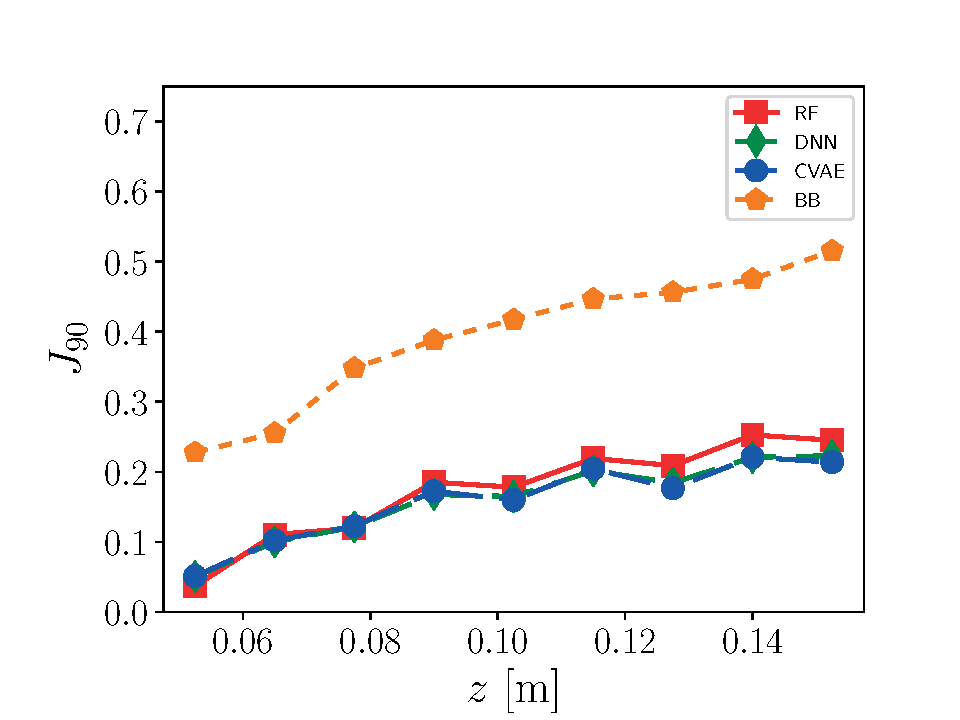
\includegraphics[page=1,width=\textwidth]{./figs/dice_predictions_skip.pdf}%
  \end{subfigure}\hfill%
  \begin{subfigure}[t]{0.48\textwidth}%
    \includegraphics[page=2,width=\textwidth]{./figs/dice_predictions_skip.pdf}%
  \end{subfigure}%
\end{figure}%
}

% ================================================================================
% Conclusions
\frame{
  \frametitle{Deep learning algorithms achieve high accuracy and low model costs.}
  \vspace*{0.3cm}
  \structure{We explored different ML techniques for PDF modeling}\\
  \hspace*{1cm}Traditional ensemble methods (random forests)\\
  \hspace*{1cm}Deep learning methods (fully connected deep neural network)\\
  \hspace*{1cm}Unsupervised, generative learning (variational autoencoder)\\[0.3cm]
  \structure{Results show that, for this study,}\\
  \hspace{1cm}ML models accurately capture PDF complexity\\
  \hspace{1cm}DL models are accurate, are fast predictors, and are small\\
  \hspace{1cm}Generative learning do not present an advantage\\
  \hspace{1cm}Analytical models present reduced accuracy\\[0.3cm]
  \structure{Future work:} \textit{a-posteriori} testing and extend to different flames\\[0.3cm]
  %\structure{Full paper can be found at URL}\\[0.3cm]
  {\tiny\textit{This research was supported by the Exascale Computing Project (ECP), Project Number: 17-SC-20-SC, a collaborative effort of two DOE organizations -- the Office of Science and the National Nuclear Security Administration -- responsible for the planning and preparation of a capable exascale ecosystem -- including software, applications, hardware, advanced system engineering, and early testbed platforms -- to support the nation's exascale computing imperative.}\par}
}

% % =================================================================================
% % Bibliography
% \begin{frame}[allowframebreaks,plain]{Bibliography}
%   \tiny
%   \bibliographystyle{model1-num-names}
%   %\bibliographystyle{jap}
%   %\bibliography{./library}
% \end{frame}

\egroup

\end{document}
